% !TEX TS-program = lualatex
% !TeX program = lualatex
% !TEX encoding = UTF-8 Unicode
% Original sample text prepared for the TeXShop website screenshot.
\documentclass[11pt,a4paper]{article}
\usepackage{fontspec}
\setmainfont{lmroman10-regular.otf}[
  BoldFont=lmroman10-bold.otf,
  ItalicFont=lmroman10-italic.otf,
  BoldItalicFont=lmroman10-bolditalic.otf
]
\usepackage[english]{babel}
\usepackage{amsmath,amssymb}
\usepackage{pgfplots}
\pgfplotsset{compat=1.18}
\usepackage[margin=23mm]{geometry}
\usepackage{microtype}
\usepackage[hidelinks]{hyperref}
\hypersetup{pdftitle={From Waves to Fourier Series}}
\setlength{\parindent}{0pt}
\setlength{\parskip}{0.45em}

\begin{document}
\begin{center}
  {\LARGE From Waves to Fourier Series}\\[0.5em]
  {\small A short mathematical note}
\end{center}

\section{Building a function from waves}
A complicated signal can often be understood as a combination
of simple oscillations. For a function with period $2\pi$,
its Fourier series takes the form
\begin{equation}
  f(x) \sim \frac{a_0}{2}
  + \sum_{n=1}^{\infty}
    \bigl(a_n\cos nx + b_n\sin nx\bigr),
\end{equation}
where the coefficients are determined by
\begin{equation}
  a_n = \frac{1}{\pi}\int_{-\pi}^{\pi}f(x)\cos nx\,dx,
  \qquad
  b_n = \frac{1}{\pi}\int_{-\pi}^{\pi}f(x)\sin nx\,dx.
\end{equation}

\section{Approximating a square wave}
For the odd square wave, defined by $f(x)=-1$ on $(-\pi,0)$
and $f(x)=1$ on $(0,\pi)$, the cosine terms vanish.
The first $N$ nonzero terms give the approximation
\begin{equation}
  S_N(x)=\frac{4}{\pi}\sum_{k=0}^{N-1}
  \frac{\sin\bigl((2k+1)x\bigr)}{2k+1}.
\end{equation}

\begin{center}
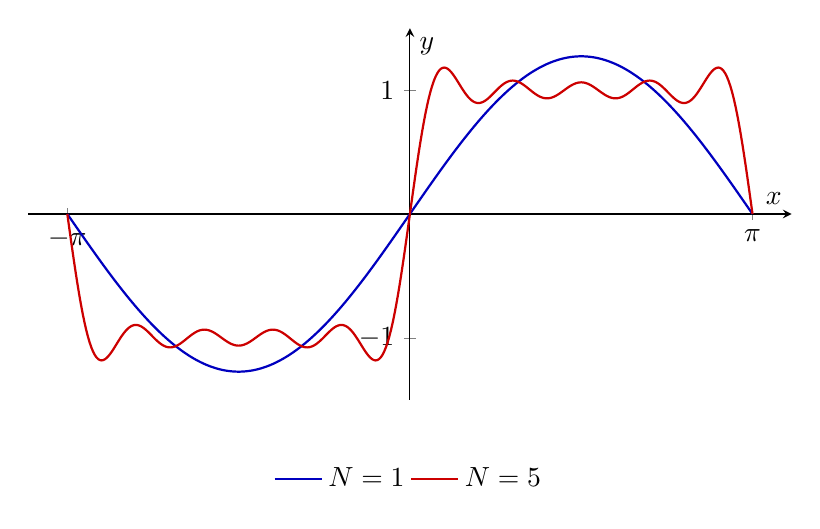
\begin{tikzpicture}
\begin{axis}[
  width=0.93\linewidth, height=6.3cm,
  axis lines=middle, xlabel={$x$}, ylabel={$y$},
  xmin=-3.5, xmax=3.5, ymin=-1.5, ymax=1.5,
  xtick={-3.14159265,0,3.14159265},
  xticklabels={$-\pi$,$0$,$\pi$}, ytick={-1,1},
  samples=401, domain=-pi:pi,
  legend style={at={(0.5,-0.15)}, anchor=north,
    draw=none, legend columns=2},
  every axis plot/.append style={thick}
]
\addplot[blue!75!black] {4/pi*sin(deg(x))};
\addlegendentry{$N=1$}
\addplot[red!80!black]
  {4/pi*(sin(deg(x))+sin(deg(3*x))/3+sin(deg(5*x))/5
        +sin(deg(7*x))/7+sin(deg(9*x))/9)};
\addlegendentry{$N=5$}
\end{axis}
\end{tikzpicture}
\end{center}

Adding more terms improves the approximation away from the jumps.
Near each discontinuity, a persistent overshoot remains:
this is the \emph{Gibbs phenomenon}.
\end{document}
